\chapter{Electroconvection}\label{ch_ele}
The term ``Electroconvection'' refers to the phenomena that occurs when a moving electrically susceptible fluid
is subjected to an applied electric field. Various geometries have been considered in the literature including, rectangular~\cite{linearstability,WNAEISFF,pattern}, annular~\cite{Annular}, and sheared annular~\cite{EDCTAFUCF,BAEWIS,SBSAE,AEWSDaDe}.
In this thesis, we consider this last case. In particular, we consider an experiment that involves a thin conductive crystal fluid in the Smectic~A phase suspended between two concentric annular electrodes. The inner electrode is rotated at a constant speed $\omega_{i}$, imposing a radial shear, and a DC voltage $V$ is applied between the two electrodes. This chapter presents an overview of the experiment of sheared annular electroconvection  and the governing equations that model it. In Section~\ref{sec_num_sol}, we present a brief overview of the simulation code that will be used in the numerical bifurcation method; for more details about the code and its implementation, we refer the reader elsewhere~\cite{PeiChunTsain}.

\section{The Physical Experiment}\label{sec_phy_exp}
We begin by introducing the experiment of Morris~et~al.~\cite{AEWSDaDe}; we include a brief description of its procedure and apparatus which has been designed to perform current-voltage measurements of electroconvection in annular liquid crystal films.
The experiment consists of observing a weakly conducting, sub-micron thick, liquid crystal film freely suspended between two concentric electrodes as the control parameters are varied. The entire set up is enclosed in an aluminum box which serves as a Faraday cage to reduce external electric interference. In the experiment setup, a razor blade controlled by a motor draws the film across the annular gap, and the electrodes are made concentric and levelled by a translation of the stage on which the fluid is suspended, by tilting adjustment rods, respectively.
Using a high precision electrometer controlled by a computer, a DC voltage $V$ is imposed across the electrodes and the resulting current $I$ is measured.
The main interest of the experiment is to study the charge transport by measuring the current $I$  as the fluid undergoes transitions as the voltage $V$ is varied.

\subsection{The fluid material}
The fluid used in the experiment is 8CB (4-cyano-4'octylbiphenyl)~\cite{AEWSDaDe}. Below $21.5^{\circ}$C, 8CB exhibits the spatial structure of a solid crystal with long-range positional and rotational order, while at temperatures higher than $40.5^{\circ}$C, the compound becomes spatially randomized and behaves as a liquid. Between these temperatures, 8CB exhibits a liquid crystal state. A schematic of the chemical formula of the fluid and the phases that it exhibits at different temperature is illustrated in Figure~\ref{8CB}, and the molecular arrangements are shown in Figure~\ref{smectic}.
Liquid crystal matter can be classified depending on the amount of order in the material~\cite{book2012liquid}. Between the temperatures $33.5^\circ$C and $40.5^{\circ}$C, 8CB exhibits a nematic phase characterized by molecules with no positional order but that point in the same direction. At lower temperatures, between $21.5^{\circ}$C and $33.5^{\circ}$C, the material enters a Smectic~A phase, where a degree of translational order is present.  In this phase, the molecules are maintained in a general orientation normal to the plane of the film and align themselves in an integer number of layers. Between the layers, motion is restricted. However, within each layer, the oriented molecules are free to move with no long-range order. Thus, each layer acts as a two-dimensional fluid.

\begin{figure}[tbh]
\centerline{\includegraphics[width =0.9\textwidth]{./figures/Pictures/8CB.png}}
\caption{Chemical formula and phase sequence of 8CB as its temperature changes.}
\label{8CB}
%[Chemical formula of 4-cyano-4'octylbiphenyl (8CB)]
\end{figure}

\begin{figure}[tbh]
%\centerline{\includegraphics[width =0.25\textwidth, keepaspectratio]{./figures/smecticphase.png}}
\centerline{\includegraphics[width =0.9\textwidth]{./figures/Pictures/liquid_crystal.png}}
\caption{Illustration of the liquid crystal that form the nematic (b) and smectic (c) phases upon cooling from the isotropic liquid (a) and above the crystal structure (d), adapted from~\cite{book2012liquid}.}
\label{smectic}
%[Changes of liquid crystal phase as temperature varies]
%\caption{shows the liquid crystal molecules in smectic-A phase. The molecules on an average are aligned in an integer number of layers with a particular normal direction. }
\end{figure}

The experiments which we will study  were conducted at room temperature $24\pm 2^{\circ}$C and atmospheric pressure. Thus the compound 8CB is in the Smectic~A phase.

\subsection{Experimental results}
A standard experiment consists of incrementing the applied voltage from $0$ volts to $1000$ volts and then decrementing it back to $0$ volts in small steps, with the inner anode rotating at a prescribed constant angular speed $\omega_i$ and the outer cathode stationary and grounded. For the range of rotation rate used in the experiments, the fluid is axisymmetric for relatively low voltage. In this state, the velocity is in the azimuthal direction where the flow lines are concentric circles and the charge diffuses between the electrodes by conduction. However, when the applied voltage $V$ exceeds a critical voltage $V_c$, the fluid becomes arranged into convective pairs of symmetric vortices, and the flow of electric charge between the electrodes constitutes a convective electric current. A snapshot of the fluid in these two states is illustrated in Figure~\ref{fig_exp_snap}.
At higher voltages $V > V_c$, a more complicated flow is provoked which retains large-scale structure of the convecting vortices. Thus, quantitative data are obtained, analysed and subsequently interpreted from raw experimental current-voltage measurements.
\begin{figure}[th]
\begin{center}
\subfigure{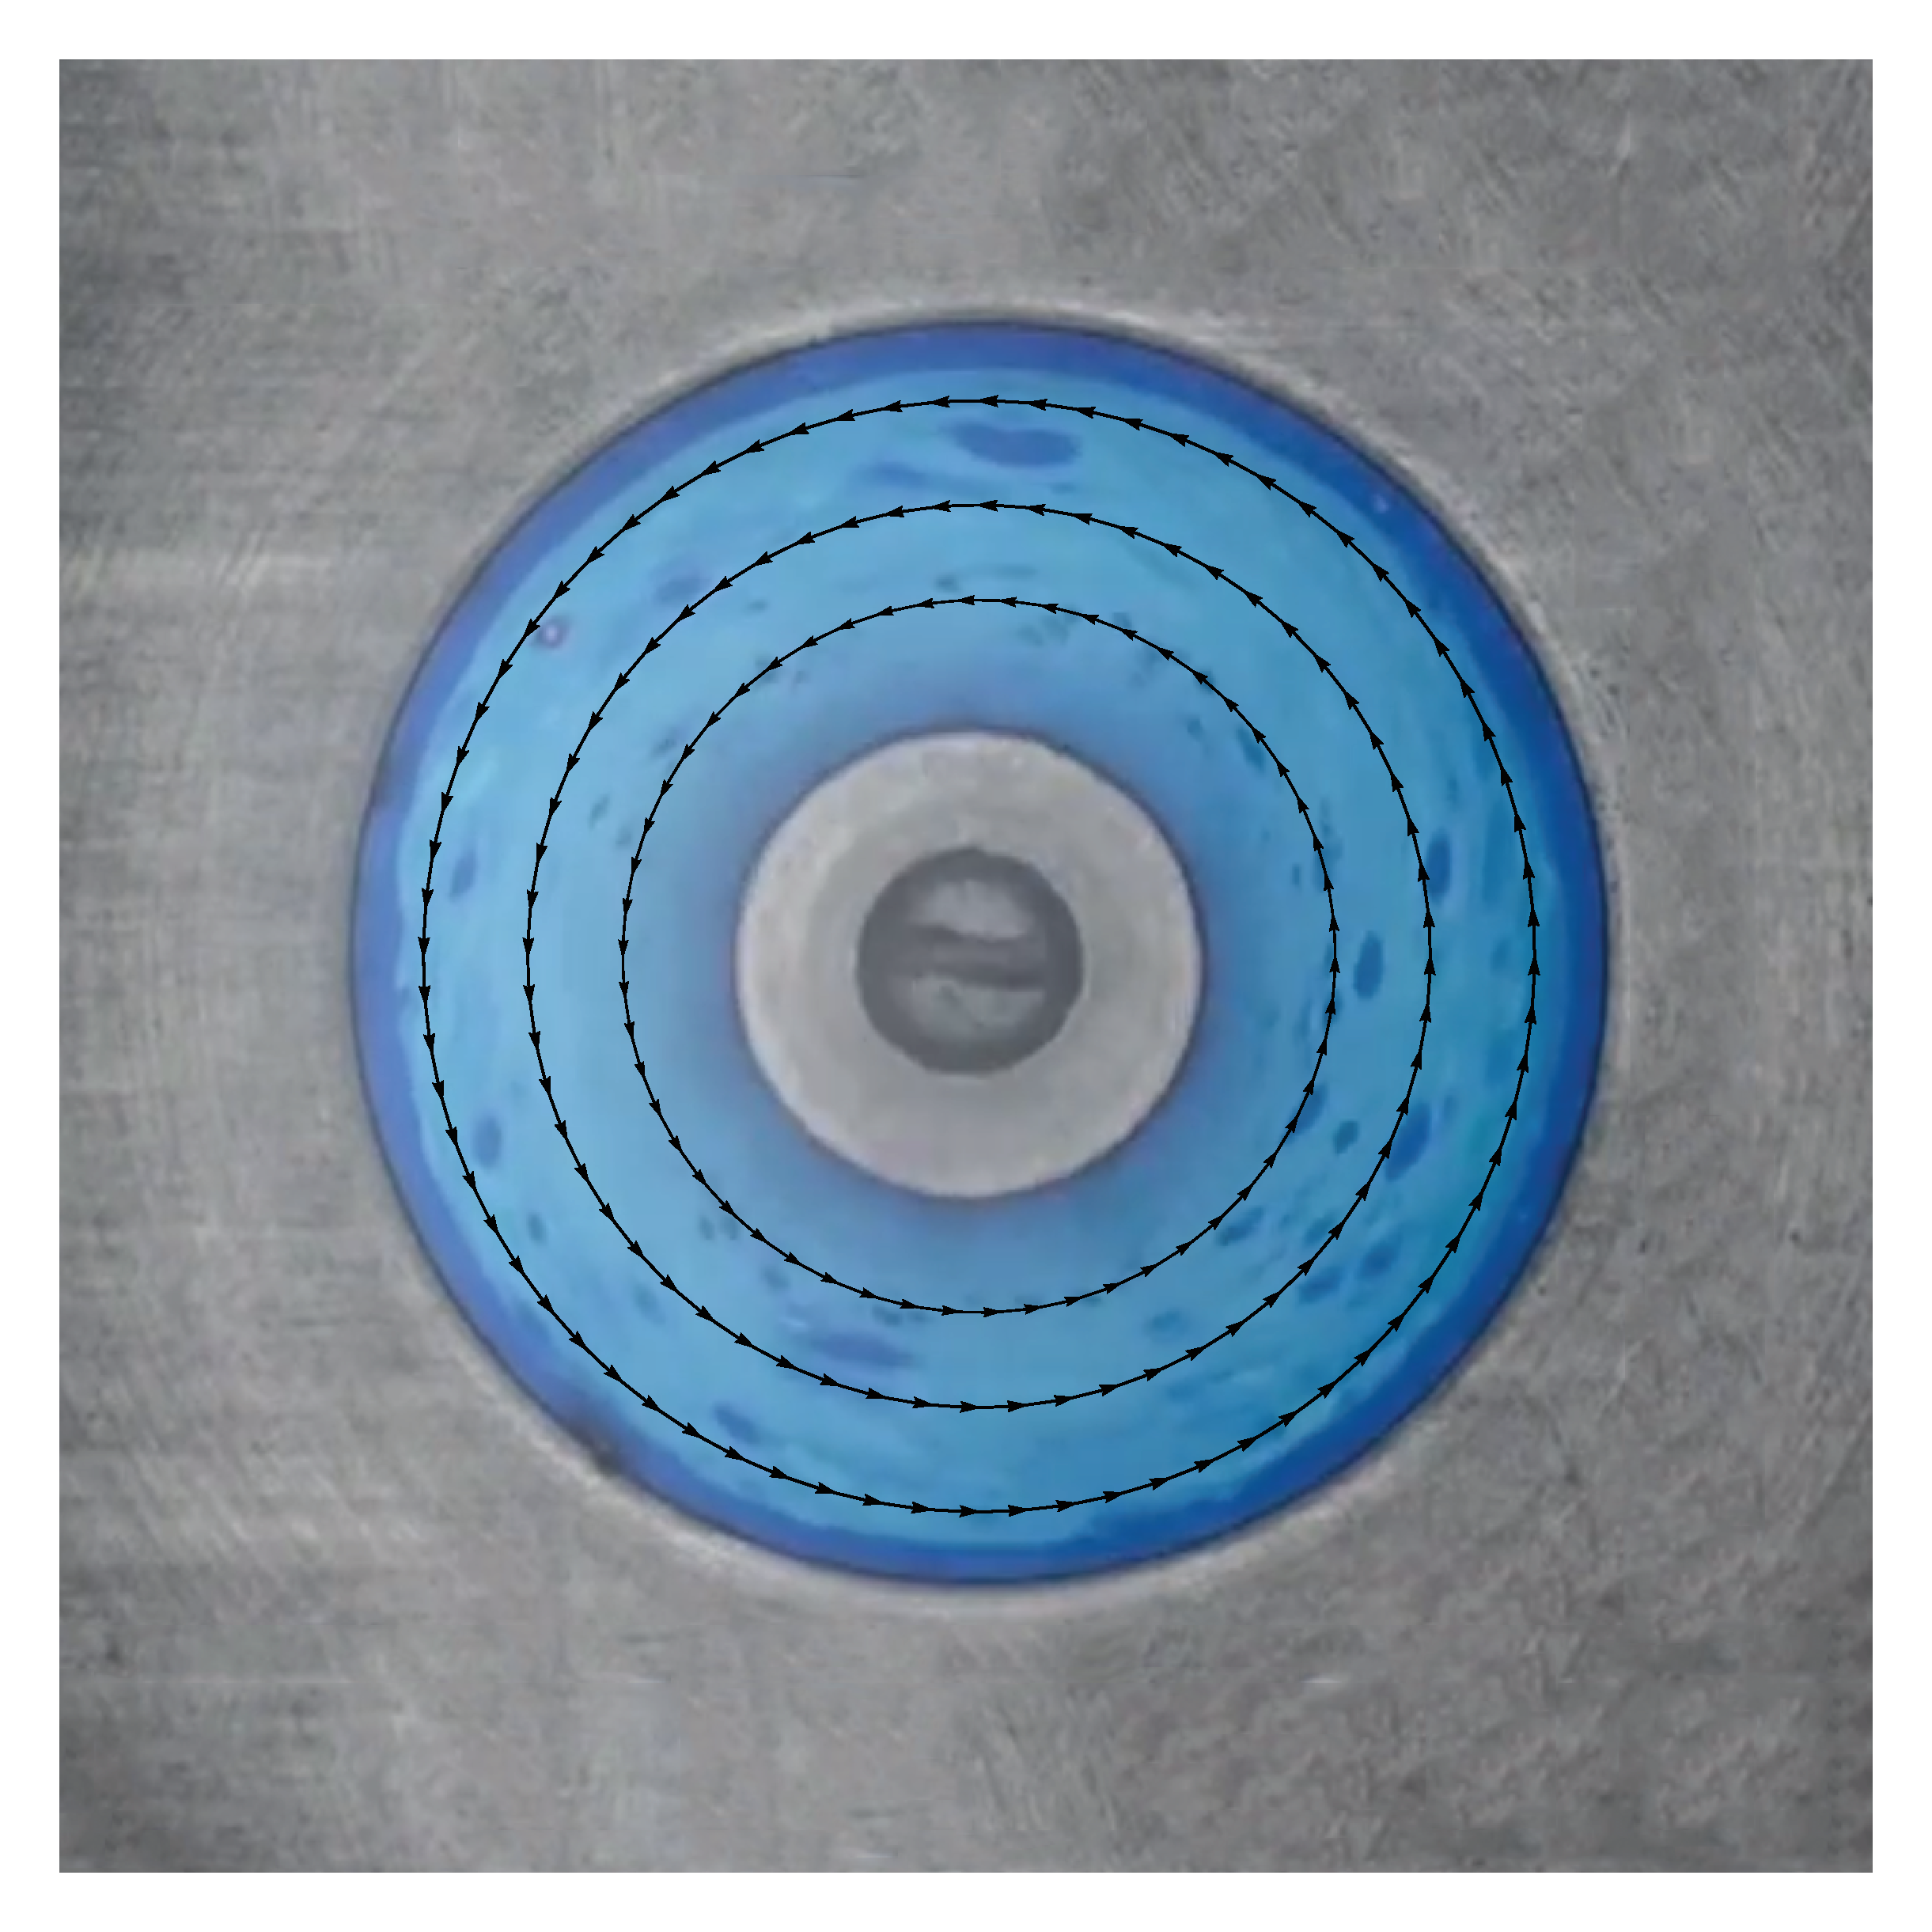
\includegraphics[width= .45\textwidth]{./figures/Pictures/physical_experiment_axi}}
\subfigure{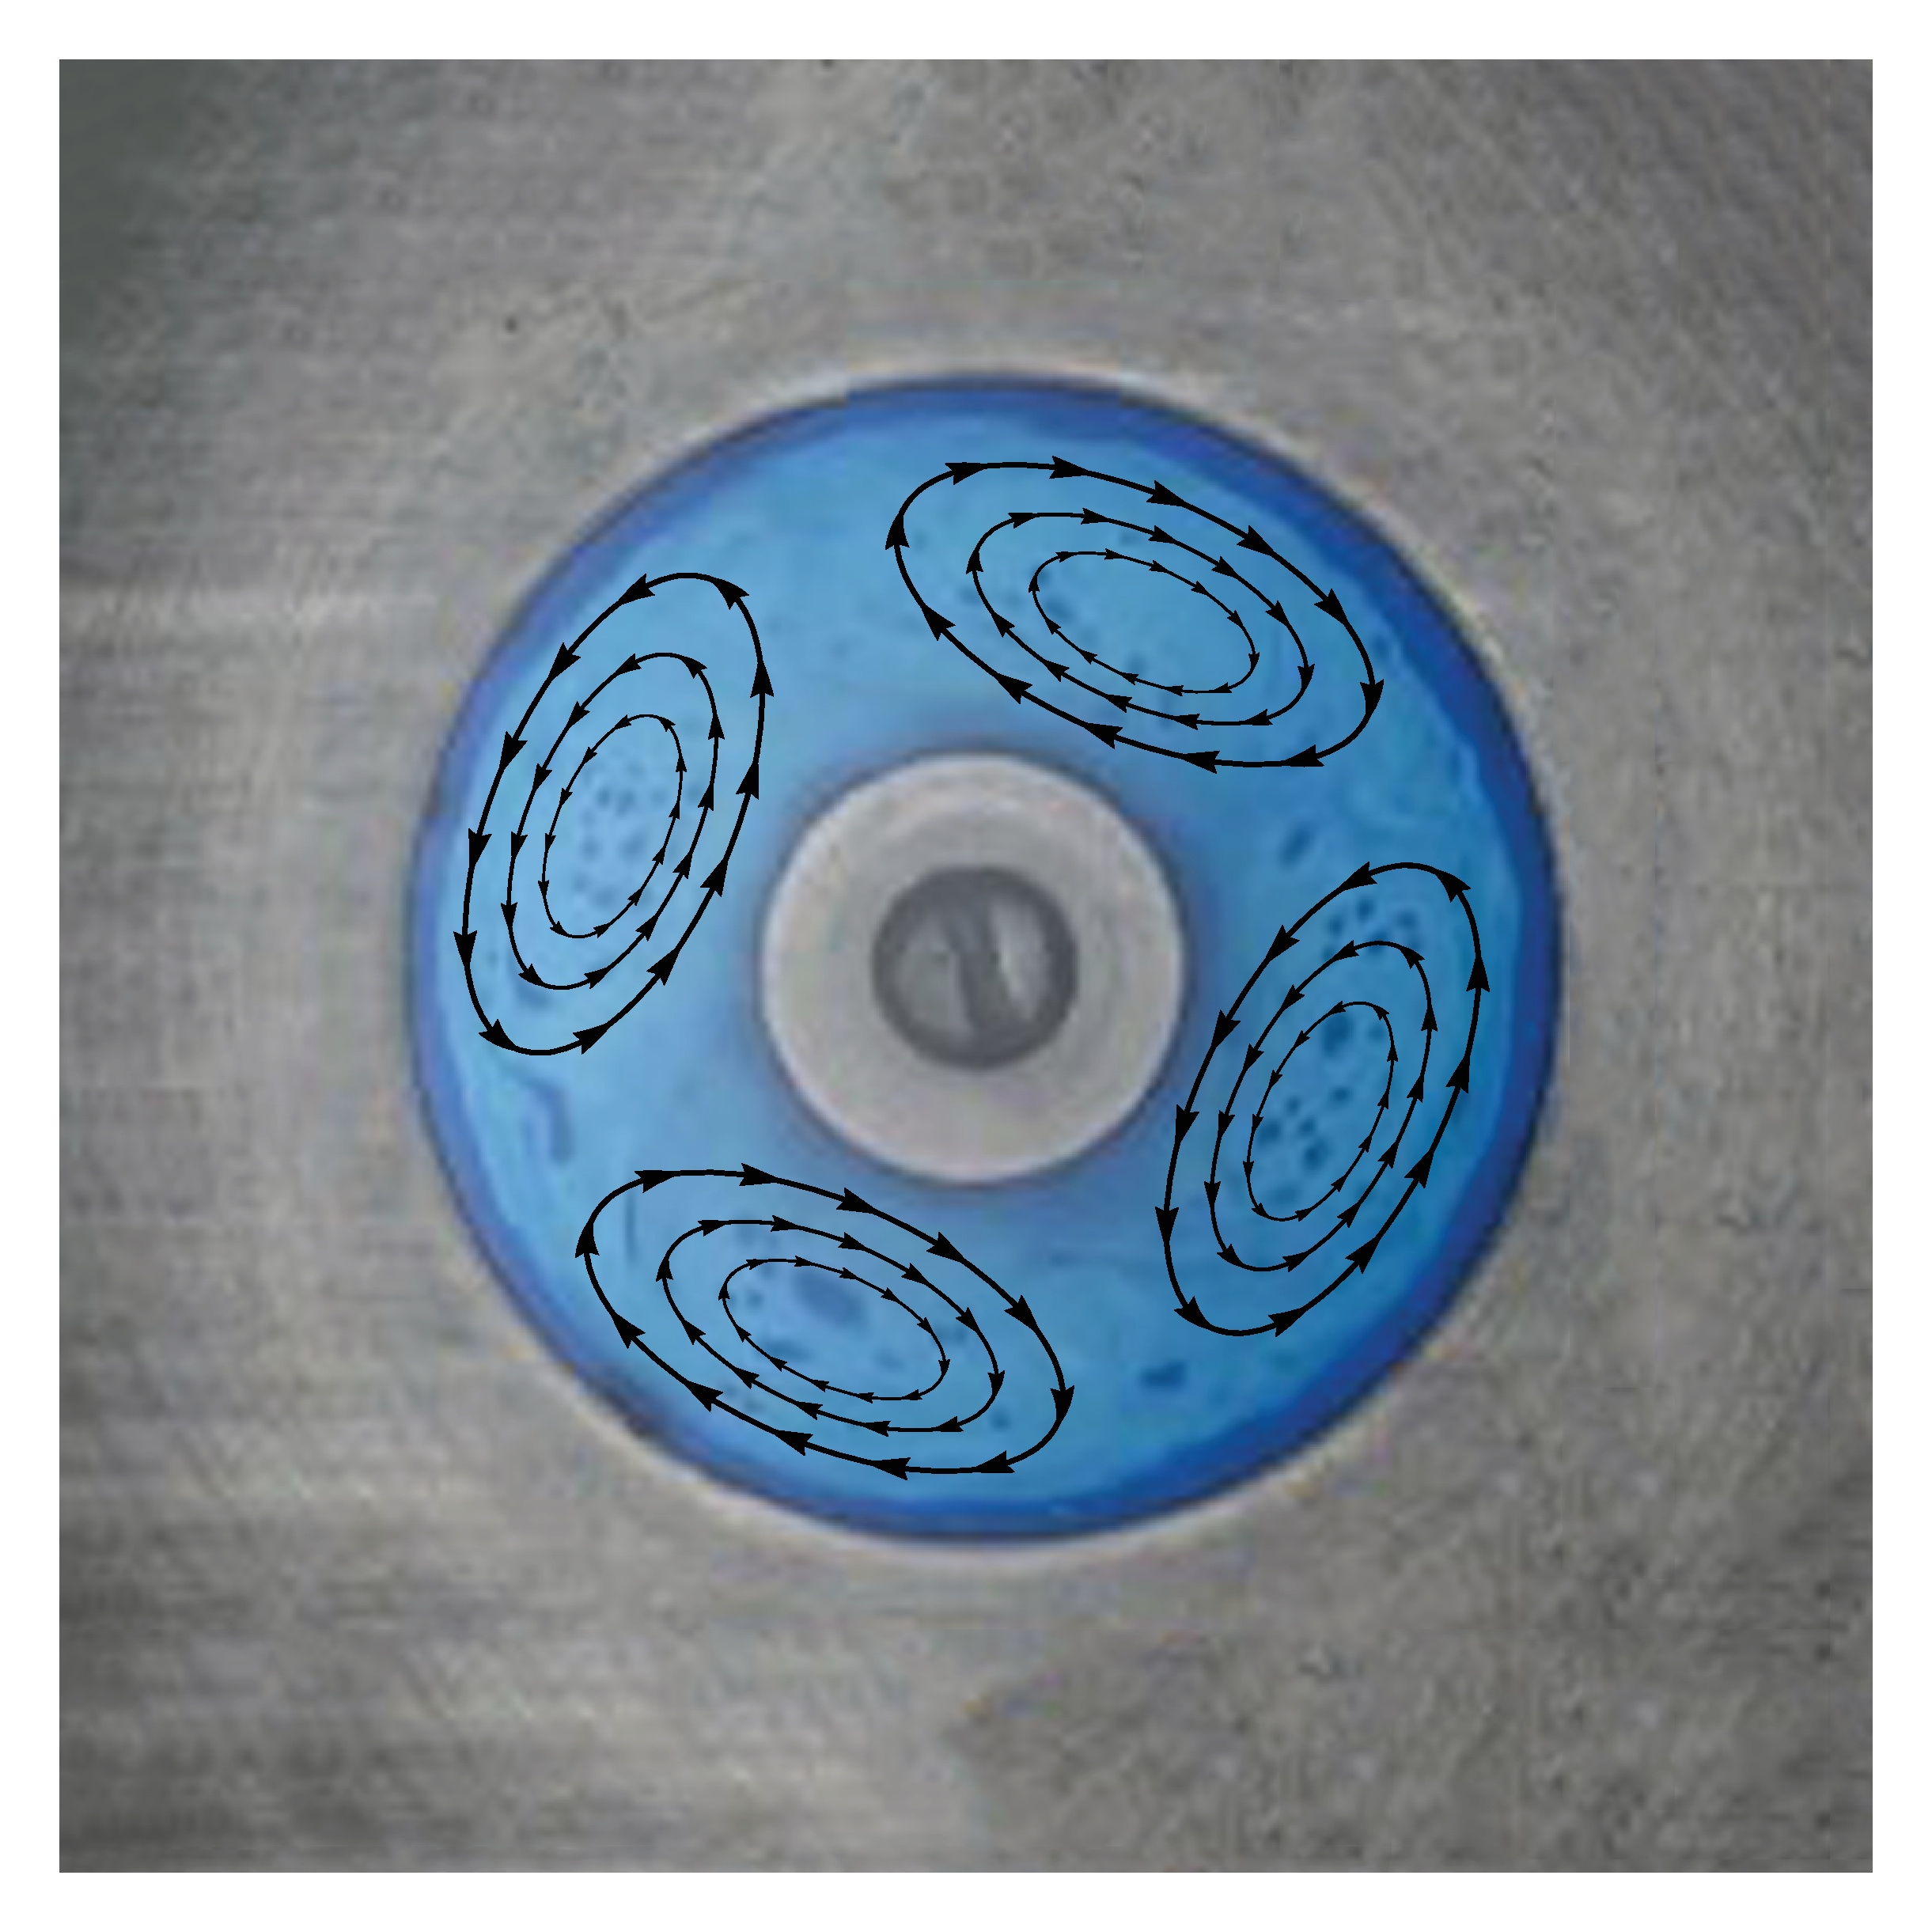
\includegraphics[width=.45\textwidth]{./figures/Pictures/physical_experiment_rotating}}
\caption{Snapshot of the two states that the flow exhibits in the physical experiment as the voltage is gradually increased between the boundaries, axisymmetric flow (left) and rotating wave flow (right). The axisymmetric flow is independent in time but the rotating wave pattern as shown in the snapshot rotates with respect to the boundaries; picture is adapted from \url{https://www.youtube.com/watch?v=WK5jRHR6NIg}. }\label{fig_exp_snap}
%[Snapshot of the axisymmetric and rotating waves flow in the physical experiment]
\end{center}
\end{figure}

As the applied voltage is incremented and then decremented in a small steps, $100$ current measurements spaced by $25$\ ms are performed and the average values of these measurements are used to calculate the Nusselt number $\mathrm{Nu}$, which is a dimensionless parameter defined as the ratio of total current to the conductive current. An Analysis of the data identified the critical voltage $V_c$ to be close to $40$ volts; at $V_c$, a primary transition from conduction to convection occurs. At $V < V_c$, the fluid flow is steady and charge was carried by ohmic conduction. For small $V>V_c$, the film flows in a series of counter-rotating pairs of laminar vortices. At $V\sim 200$ volts, a secondary transition was identified due to a sudden jump in the current fluctuations. At even higher voltages $V \gtrsim 600$ volts, the flow becomes turbulent.

This experiment has been repeated for different constant angular speeds of the inner electrodes to investigate the effect of the rotation on the primary transition. It is shown in~\cite{BAEWIS,AEWSDaDe}, that the primary transition is supercritical for different rotation rates, i.e. the amplitude of the convective vortices grow monotonically from zero. Furthermore, the rotation acts as a stabilizer of the flow, delaying the onset of convection.
These transitions can be reproduced with the numerical simulations of the mathematical model which we describe next.
%The limitations of the physical experimentation lead to another approach, that is, studying a mathematical model that copy the experiment.

\section{The Mathematical Model}\label{sec_mat_mod}
For the model, we assume that the film is confined between two concentric annular electrodes as shown in Figure~\ref{experiment_diagram}. An electric potential difference is applied between the boundaries with the inner electrode rotating at a constant angular speed. This section discusses the mathematical model describing the physical experiment and the base state solution of the governing equations. A brief overview of the pseudo-spectral numerical method, used to solve the perturbation equations from the base state, is also discussed.

\begin{figure}[t]
\centering{\includegraphics[width = .45\textwidth]{./figures/Pictures/ele_con_pic1}}
\caption{Relevant geometry of sheared annular electroconvection.}
\label{experiment_diagram}
%[Illustration of the experiment of annular electroconvection]
\end{figure}

\subsection{The governing equations}\label{sec_gov_equ}
In this section, the governing equations and the boundary conditions that model the experiment of annular electroconvection are presented. In the physical experiment, the thin film is confined in an annular region defined in cylindrical coordinates as, $r_i\le r\le r_o$. The film is a liquid crystal in Smectic~A phase with thickness $s$,  much smaller than the gap width $d = r_o-r_i,$ such that $d\gg s$. Considering this and the property of Smectic~A phase that inhibits motion between layers, we assume that the film can be considered as a 2D electrically conducting Newtonian fluid in the plane $z=0$. The density, viscosity and conductivity of the fluid are denoted by $\rho, \eta$ and $\sigma$ respectively. The inner electrode, $0\le r\le r_i$, is rotating at a constant angular speed $\omega_i$ and is held at an electric potential $V$. The outer electrode, $ r\ge r_o$, is held at zero potential and does not rotate. The conservation of momentum and the conservation of matter, given by the incompressible Navier-Stokes equations with an electric body force $q\mathbf{E}$, model the velocity field $\mathbf{u}(r,\theta,t) = u(r,\theta,t) \hat{\mathbf{r}} + v(r,\theta,t) \boldsymbol{\hat{\theta}}$
\begin{subequations}
\begin{align}
\label{Nav_Sto}
&\rho\left(\pderiv[]{\mathbf{u}}{t} + \left(\mathbf{u}\cdot\nabla\right)\mathbf{u}\right) = -\nabla P + \eta\nabla^2\mathbf{u} + q\mathbf{E},\\
\label{Incompress}
&\nabla\cdot\mathbf{u} = 0,
\end{align}
where $\hat{\mathbf{r}}$ is the unit vector in the radial direction, $\boldsymbol{\hat{\theta}}$ is the unit vector in the azimuthal direction, $\nabla$ is the 2D gradient operator, $P$ is the pressure,  $q$ is the surface charge density, $\mathbf{E} = -\left(\nabla\psi\right)|_{z=0}$ is the electric field in the film plane $z = 0$ and $\psi$ is the 3D electric potential.  The conservation of charge is expressed by the continuity equation
\begin{align}
\label{charge_con}
\pd{q}{t} = -\nabla\cdot \mathbf{J}, \hspace{1cm} \mathbf{J} = \sigma\mathbf{E} + q\mathbf{u},
\end{align}
where the current density $\mathbf{J}$ is composed of a term due to ohmic conduction density $\sigma\mathbf{E}$ and a term due to the fluid convection $q\mathbf{u}$. The electric potential $\psi$ satisfies the Laplace equation
\begin{align}
\label{laplace_eq}
\lb \nabla^2 + \pderiv[2]{}{z}\rb\psi = 0,
\end{align}
in the charge free region $z\ne 0$. To find the charge in the film region $z =0$, we note that by assuming that any magnetic effects are neglected, the 2D surface charge density $q$ satisfies Maxwell's equation~\cite{linearstability}
\begin{align}
\label{Maxwell_relation}
q = -2\epsilon_0 \pderiv{\psi}{z}\Big{|}_{z=0^+},
\end{align}
where $\epsilon_0$ is the permittivity of free space.
\end{subequations}
%The Maxwell's equation is presented by  which describes a nonlocal relation between the surface charge density and the 3D electric potential $\psi$. Therefore, in the space $z\ne0$, that is free of charge, the 3D electric potential satisfy Laplace equation,
%\begin{align}
%\label{laplace_eq}
%\lb \nabla^2 + \pderiv[2]{}{z}\rb\psi = 0.
%\end{align}

Equation ~(\ref{Nav_Sto})--(\ref{Maxwell_relation}) are subject to the following boundary conditions.
The velocity field satisfies no-slip boundary conditions
\begin{subequations}
\begin{align}
&\mathbf{u} = \omega_i r_i \boldsymbol{\hat{\theta}}, &  & r = r_i,\\
&\mathbf{u} = 0, & & r = r_o,
\end{align}
at each electrode.
The potential $\psi$ is set to zero at infinity
\begin{align}
\lim_{z \to \pm \infty} \psi(r,\theta,z) = 0,
\end{align}
and, at $z = 0$, takes on the imposed voltage, so that
 \begin{equation}
    \psi(r,\theta,0)= \psi_2(r,\theta) =
\begin{cases}
    V,& \text{for } r \le r_i,\\
    0,              & \text{for } r\ge r_o,
\end{cases}
\end{equation}
\end{subequations}
where $\psi_2$ is the 2D electric potential in the fluid plane.

A streamfunction-vorticity formulation can be used to eliminate the pressure term, where the fluid velocity field is replaced by two scalar function $\omega$ and $\phi$ defined as follows
\begin{align}
\label{stream}
\mathbf{u} &= \nabla\phi\times\hat{\mathbf{z}}, & \nabla\times\mathbf{u} &= \omega\hat{\mathbf{z}},
\end{align}
where $\omega = \omega(r,\theta,t)$ and $\phi = \phi(r,\theta,t)$ are the vorticity and streamfunction of the flow, respectively. In addition, we can define a characteristic length, time and charge. If we let the imposed voltage $V$ denote a representative voltage over a length scale of size $d = r_o - r_i$ and a relaxation time $\tau_c = \epsilon_0 d/\sigma$, where $\sigma$ is the conductivity and $\epsilon_0$ is the permeability constant, then we obtain the following natural nondimensionalization
\begin{align}
\label{nondimes}
r &= d \tilde{r},     & \phi &= \frac{\sigma d}{\epsilon_0}\tilde\phi, &  \psi &= V\tilde{\psi} & t &= \tau_c\tilde{t}, & q & = \frac{\epsilon_0 V}{d}\tilde{q},
\end{align}
where the tilde represents the dimensionless variables.
Applying the formulation~(\ref{stream}) to~(\ref{Nav_Sto})--(\ref{Maxwell_relation}), nondimensionalizing with~(\ref{nondimes}) and dropping the tilde, we obtain the system of equations describing the evolution of the dimensionless physical quantities, vorticity $\omega$, streamfunction $\phi$, charge density $q$, the 2D potential in the fluid $\psi_2$ and the 3D potential $\psi$,
\begin{subequations}
\begin{align}
\label{dim_less_1}
&\nabla^2\phi = -\omega, \\
\label{dim_less_2}
&\pd{\omega}{t}+\lb \mathbf{u}\cdot\nabla\rb\omega =\mathcal{P}\nabla^2\omega + \mathcal{PR}\lb \nabla\psi_2\times\nabla q\rb\cdot\mathbf{\hat{z}},\\
&\pd{q}{t}+\lb \mathbf{u}\cdot\nabla\rb q = \nabla^2\psi_2,\\
&\lb \nabla^2 + \pderiv[2]{}{z}\rb\psi = 0, \hspace{2cm} q = -2\pd{\psi}{z}\Big{|}_{z=0^+}, \label{dim_less_end}
\end{align}
\end{subequations}
where the nondimensional parameter groups are the Rayleigh number $\mathcal{R}$ and the Prandlt number $\mathcal{P}$ defined as
\begin{align}
 \mathcal{R} &= \frac{\epsilon_{0}^2V^2}{\sigma\eta}, & \mathcal{P} &= \frac{\epsilon_{0}\eta}{\rho\sigma d},
\end{align}
respectively.
The Rayleigh number $\mathcal{R}$, which is proportional to the square of the applied voltage $V$, describes the relative strength of the applied electric forcing to the viscous dissipation, and the Prandlt number $\mathcal{P}$ is a fluid parameter that describes the ratio of the charge relaxation time to the viscous relaxation time.

The boundary conditions also transform and become
\begin{subequations}
\begin{align}
\label{bcd_1}
&\pderiv[]{}{r}\phi(r_o,\theta)= 0, &  &\pderiv[]{}{\theta}\phi(r_o,\theta) = 0,\\
&\pderiv[]{}{r}\phi(r_i,\theta)= -\frac{\omega r_i \epsilon_0}{\sigma} = -\omega_i r_i \tau_c,& &\pderiv[]{}{\theta}\phi(r_i,\theta) = 0,\\
& \psi_2(r_i,\theta) = 1,    &    &\psi_2(r_o,\theta) = 0,
\end{align}
\begin{equation}
    \psi(r,\theta,0)=
\begin{cases}
    1,& \text{for } 0\le r \le r_i,\\
    \psi_2(r,\theta), & \text{for } r_i\le r \le r_o,\\
    0,              & \text{for } r\ge r_o,
\end{cases}
\end{equation}
\begin{equation}
\label{bc_dim_end}
\lim_{z \to \pm \infty} \psi(r,\theta,z) = 0,
\end{equation}
\end{subequations}
where $r_i, r_o$ are dimensionless quantities scaled by $d$ and the the tilde have once again been dropped for clarity.
The cross width of the film in dimensionless units is then, $r_o-r_i = 1$, where $r_o$ is the dimensionless radius of the outer electrode set at zero electric potential and $r_i$ is the dimensionless radius of the inner electrode set at an electric potential of 1. It is convenient to express the radii of the annular geometry with the aspect ratio $\alpha = r_i/r_o$. Introducing this, the dimensionless radii can be express as
\begin{align}
\label{aspect_ratio}
r_{i} & = \frac{\alpha}{1- \alpha}, &  r_o & = \frac{1}{1- \alpha}.
\end{align}

Equations~(\ref{dim_less_1})--(\ref{dim_less_end}) with the boundary conditions~(\ref{bcd_1})--(\ref{bc_dim_end}) describe the sheared annular electroconvection of any arrangement of 2D thin conductive film freely suspended in empty space. In other words, the model still holds for the unsheared electroconvection with appropriate changes to the boundary conditions.


\subsection{The perturbation equations}
The governing equations introduced in the previous section are now solved for the case of sheared annular electroconvection. Cylindrical coordinates $(r,\theta,z)$ are employed, where $z = 0$ is defined to be the plane in which the film is suspended between the two circular electrodes.
At very low rotation rates, an axisymmetric flow is observed. We call this flow the base state and denote it by a superscript zero. This flow can be computed analytically as follows.
With the rotation of the inner electrode generating a steady Couette shear described by the dimensionless Reynolds number
\begin{align}
\mathrm{Re} = \frac{r_i\Omega}{\mathcal{P}},
\end{align}
where $\Omega = \tau_{c}\omega_i$ is the dimensionless angular frequency of the inner electrode,
 the radial derivative of the base state streamfunction and the vorticity~\cite{EDCTAFUCF} can be obtained from
%The rotation of the inner electrodes generates a Couette shear in the base state that we denote with a superscript zero. The base state of the streamfunction and the vorticity given an imposed shear is obtained by,
\begin{align}
\label{base_phi}
\pderiv[]{\phi^{(0)}(r)}{r} &= \frac{\alpha^2\Omega}{1-\alpha^2}\left( r-\frac{1}{r(1-\alpha)^2}\right),\\
%\end{align}
%\begin{align}
\label{base_omega}
 \omega^{0}(r) &= 0.
\end{align}
The base state of the charge density and the potential can also be solved analytically and one can verify that
\begin{align}
\label{base_q}
q^{(0)}(r) = \frac{2}{\ln{\alpha}}\left( \frac{1}{r}F\left(\frac{1}{2},\frac{1}{2};1;\frac{r_o^2}{r^2}\right) - \frac{1}{r_i}F\left(\frac{1}{2},\frac{1}{2};1;\frac{r^2}{r_i^2}\right)\right)
\end{align}
\begin{equation}
\label{base_psi2}
    \psi_2^{(0)}(r)=
\begin{cases}
    1,& \text{for } 0\le r \le r_i,\\
    \frac{1}{\ln{\alpha}}\left(\ln{(1-\alpha)} + \ln{r}\right), & \text{for } r_i\le r \le r_o,\\
    0,              & \text{for } r\ge r_o,
\end{cases}
\end{equation}
\begin{equation}
\label{base_psi}
\psi^{(0)}(r,z) = \int_0^\infty A(k)J_0(kr)e^{-kz} \text{d}k
\end{equation}
where $F$ is a hypergeometric function~\cite{EDCTAFUCF}, $J_0$ is the zeroth Bessel function and
\begin{align}
A(k) = k\int_0^\infty \psi^{(0)}(r,0)J_0(kr)r\text{d}r.
\end{align}
We note that, in this experiment, the inner electrodes is rotating at a constant rate while the outer electrodes is fixed.  However, independent rotations of the electrodes can be dealt by applying a transformation to a rotating frame of reference, where the outer electrode is stationary. The Coriolis forces introduced by the transformation can be absorbed into the pressure term of~(\ref{Nav_Sto}).

We can now decompose the solutions into this base state (axisymmetric) component denoted by a superscript zero and a perturbation from the base state denoted by a superscript one so that
\begin{subequations}
\begin{align}
\phi(r,\theta,t)   = \phi^{(0)}(r)   &+ \phi^{(1)}(r,\theta,t),\\
\omega(r,\theta,t) = \omega^{(0)}(r) &+ \omega^{(1)}(r,\theta,t),\\
q(r,\theta,t)      = q^{(0)}(r)      &+ q^{(1)}(r,\theta,t),\\
\psi_2(r,\theta,t) = \psi_2^{(0)}(r) &+ \psi_2^{(1)}(r,\theta,t),\\
\psi(r,\theta,z,t) = \psi^{(0)}(r,z) &+ \psi^{(1)}(r,\theta,z,t).
\end{align}
\end{subequations}
Upon applying the decomposition of the solution into a base state and perturbation from the base state and substituting in~(\ref{dim_less_1})--(\ref{dim_less_end}), we obtain the following set of equations
\begin{subequations}
\begin{align}
\label{pert_1} &\nabla^2 \phi^{(1)} = -\omega^{(1)},\\
&\pderiv[]{q^{(1)}}{t} + \mathcal{J}_{(q,\phi)} - \nabla^2\psi_2^{(1)} = 0, \\
&\pderiv[]{\omega^{(1)}}{t} + \mathcal{J_{(\omega,\phi)}} = \mathcal{P} \nabla^2\omega^{(1)} + \mathcal{PR}\mathcal{J}_{(\psi_2,q)},\\
\label{pert_end} &\left(\nabla^2_{r\theta} + \pderiv[2]{}{z} \right)\psi^{(1)} = 0, \hspace{2cm}
q^{(1)} = -2\pderiv[]{\psi^{(1)}}{z}\Big{|}_{z=0},
\end{align}
\end{subequations}
where $\mathcal{J}_{(i,j)}$ are the nonlinear Jacobian terms
\begin{subequations}
\begin{equation}
\label{Jacobian_1}
\mathcal{J}_{(q,\phi)} = \frac{1}{r}\left(\pderiv[]{q^{(0)}}{r}\pderiv[]{\phi^{(1)}}{\theta} + \pderiv[]{q^{(1)}}{r}\pderiv[]{\phi^{(1)}}{\theta}
                                       -  \pderiv[]{\phi^{(0)}}{r}\pderiv[]{q^{(1)}}{\theta} - \pderiv[]{\phi^{(1)}}{r}\pderiv[]{q^{(1)}}{\theta}   \right),
\end{equation}
\begin{equation}
\mathcal{J}_{(\omega,\phi)} = \frac{1}{r}\left(\pderiv[]{\omega^{(0)}}{r}\pderiv[]{\phi^{(1)}}{\theta}+\pderiv[]{\omega^{(1)}}{r}\pderiv[]{\phi^{(1)}}{\theta}
                                       -  \pderiv[]{\phi^{(0)}}{r}\pderiv[]{\omega^{(1)}}{\theta} - \pderiv[]{\phi^{(1)}}{r}\pderiv[]{\omega^{(1)}}{\theta}   \right),
\end{equation}
\begin{equation}
\mathcal{J}_{(\psi_2,q)} = \frac{1}{r}\left(\pderiv[]{\psi_2^{(0)}}{r}\pderiv[]{q^{(1)}}{\theta} - \label{Jacobian_end}
\pderiv[]{q^{(0)}}{r}\pderiv[]{\psi_2^{(1)}}{\theta}
                                        + \pderiv[]{\psi_2^{(1)}}{r}\pderiv[]{q^{(1)}}{\theta} - \pderiv[]{q^{(1)}}{r}\pderiv[]{\psi_2^{(1)}}{\theta} \right).
\end{equation}
\end{subequations}
The perturbation variables $\phi^{(1)},\psi_2^{(1)}$ and $\psi^{(1)}$ must satisfy the following boundary conditions
\begin{subequations}
\begin{equation}
\phi^{(1)}(r_i,\theta) = \pderiv[]{}{r}\phi^{(1)}(r_i,\theta) =
\phi^{(1)}(r_o,\theta) = \pderiv[]{}{r}\phi^{(1)}(r_o,\theta) = 0,
\end{equation}
\begin{equation}
\psi_2^{(1)}(r_i,\theta) = \psi_2^{(1)}(r_o,\theta) = 0,
\end{equation}
\begin{equation}
    \psi^{(1)}(r,\theta,0)=
\begin{cases}
    0,& \text{for } 0\le r \le r_i,\\
    \psi_2^{(1)}(r,\theta), & \text{for } r_i\le r \le r_o,\\
    0,& \text{for } r \ge r_o,
\end{cases}
\end{equation}
\begin{equation}
\lim_{z \to \pm \infty} \psi^{(1)}(r,\theta,z) = 0.
\end{equation}
\end{subequations}
This latter set of equations determines the perturbation from the base state and its numerical solution will be considered in the subsequent sections.

\section{The Numerical Solver}\label{sec_num_sol}
In this section, we provide a brief overview of the numerical time stepper implemented in MATLAB~\cite{PeiChunTsain} that we will use for our numerical bifurcation method. The solutions of~(\ref{dim_less_1})--(\ref{dim_less_end}) are approximated with a pseudospectral method in order to take advantage of the efficiency of the Fast Fourier Transform (FFT) and the inherent convergence properties of this method~\cite{Trefethen}.
The periodic boundary conditions suggest the choice of the Fourier basis $\{e^{im\theta}\}$ in the angular coordinate and, due to the no-slip condition which leads to steep changes at the boundaries, the choice of Tchebychev basis for the radial coordinate becomes favorable to avoid Gibbs phenomenon. Thus, the 2D physical quantities, the streamfunction $\phi$, the vorticity $\omega$, the charge density $q$ and the electric potential $\psi_2$, can be approximated using a truncated Fourier series $\{e^{im\theta}\}$ in the $\boldsymbol{\hat{\theta}}$ direction and a series of Tchebychev polynomials $T_n(r)$ in the $\hat{\mathbf{r}}$ direction, that is
\begin{subequations}
\begin{align}
\phi^{(1)}(r,\theta,t) &= \sum_{n=0}^{N_c}\sum_{m = -K}^{K}\tilde{\phi}_{nm}(t)e^{im\theta}\,T_n(x),\\
\omega^{(1)}(r,\theta,t) &= \sum_{n=0}^{N_c}\sum_{m = -K}^{K}\tilde{\omega}_{nm}(t)e^{im\theta}\,T_n(x),\\
q^{(1)}(r,\theta,t) &= \sum_{n=0}^{N_c}\sum_{m = -K}^{K}\tilde{q}_{nm}(t)e^{im\theta}\,T_n(x),\\
\psi_2^{(1)}(r,\theta,t) &= \sum_{n=0}^{N_c}\sum_{m = -K}^{K}\tilde{\psi_2}_{nm}(t)e^{im\theta}\,T_n(x),
\end{align}
\end{subequations}
where $K$ is the highest Fourier mode, $N_c$ is the order of the highest Tchebychev polynomial and
\begin{align}
x = 2r - \frac{1+\alpha}{1-\alpha},
\end{align}
linearly maps $r \in \left[\frac{\alpha}{1-\alpha}, \frac{1}{1-\alpha}\right]$ to $x \in [-1,1]$ that spans the film. The reason for this remapping is to utilize the collocation points, $x_j = \cos(\pi j/N_c),\ j = 0,1,\ldots,N_c$, at which the collocation method that approximates the solution as a truncated Tchebychev polynomial series  makes the residual equal to zero.

The time-stepping was implemented in two different schemes. The first scheme is an implicit-explicit Euler method in which the linear terms are computed implicitly and the nonlinear terms are computed explicitly. Using this scheme, the time derivative is approximated as
\begin{equation}
\label{scheme_euler}
\pderiv[]{u}{t}  \approx \frac{u^{(k+1)} - u^{(k)}}{\delta t}.
\end{equation}
where $\delta t$ is a prescribed time step and $u$ is the discretized solution vector. The other scheme that is implemented uses a second-order implicit backward difference method (BDI2) in which the time derivative is approximated as
\begin{equation}
\label{BDI2}
\pderiv[]{u}{t} \approx \frac{3u^{(k+1)} -4u^{(k)}+ u^{(k-1)}}{2\delta t},
\end{equation}
and the nonlinear terms given by equations~(\ref{Jacobian_1})--(\ref{Jacobian_end}) are approximated using a first-order Adams-Bashforth method (AB$_1$).

The numerical time-stepper for the smectic electroconvection is complicated by a nonstandard boundary condition. The surface charge $q$ is not only coupled to flow motion, but also regulated by the 2D electric potential field $\psi_2$. To handle this situation, a different approach is required to resolve the nonlocal coupled electric body force that involves Maxwell's equation~(\ref{pert_end}) which connects the charge density with the electric potential. However, the nonlocal calculation of the 3D potential and the charge field are assumed to couple instantaneously and therefore do not involve any time derivatives. The Laplace equation is solved implicitly in integral form where the boundary condition is resolved by decomposing the field using a pseudospectral technique~\cite{PeiChunTsain}.

With the proper initial conditions, boundary conditions and time step, the 2D electric potential $\psi_2$ is computed simultaneously with the surface charge $q$ by means of the nonlocal mapping. The vorticity $\omega$ can then be obtained from the computed $q$ and $\psi_2$ leading to the computation of the streamfunction $\phi$. The Orszag 3/2 aliasing rule is performed when dealing with the nonlinear terms.

The two different time-stepping were used to estimate and compare the accuracy of the solutions. It was found that both implementations yield in consistent simulation results in the weakly nonlinear regime and the second scheme (AB$_1$)/(BDI2) gives second order accuracy~\cite{PeiChunTsain}. For high Rayleigh number, the second scheme was more stable and preferable where the time step $\delta t$ is limited due to computational instability. For our implementation, we use the second scheme.

The time stepper computes some extra integrated physical quantities such as a dimensionless  Nusselt number $\mathrm{Nu}$ and a mean area density of the kinetic energy. The Nusselt number is defined as  the ratio of total current to the conductive current transported by diffusion process. For more detailed explanation of the time stepper, the reader is referred to~\cite{PeiChunTsain}.

\subsection{Numerical results}
For comparative purposes with the latter part of this thesis, we highlight in this section some of the numerical results obtained in~\cite{PeiChunTsain,DNSSAE}. As in this thesis, the main control parameter of interest is the Rayleigh number $\mathcal{R}$. Long time integrations of a random initial condition are performed to study the effect of the Rayleigh number $\mathcal{R}$ on the base state solution, while fixing the other nondimensional parameters $\mathcal{P},\mathrm{Re}$ and $\alpha$. The flow undergoes a primary transition from axisymmetric to rotating waves as $\mathcal{R} > \mathcal{R}_c$. This transition is found to be a supercritical Hopf bifurcation for a wide range of dimensionless parameters $\{\mathcal{P},\alpha,\mathrm{Re}\}$. Amplitude vacillating waves are observed for higher values of $\mathcal{R}$. Further increases in $\mathcal{R}$ cause the flow to exhibit a steady convective wave state with a different integer number of vortices distinct in character from the primary transition and the flow eventually becomes turbulent for relatively large Rayleigh numbers.

The effect of the aspect ratio $\alpha$, the Prandlt number $\mathcal{P}$ and the Reynolds number $\mathrm{Re}$ on the primary transition are also investigated in~\cite{PeiChunTsain}. In particular, the critical Rayleigh number $\mathcal{R}_c$ and the critical mode $m_c$, (the number of counter rotating waves pairs) are observed for various values of these parameters. The authors find that, the aspect ratio $\alpha$ strongly influences $\mathcal{R}_c$ and $m_c$, with numerous codimension-two points observed when two critical modes $m = m_c$ and $m=m_c + 1$ become unstable. Eventually one mode saturates to a convective state and the other slowly decays.
Changes in the Prandlt number $\mathcal{P}$, which is a fluid parameter that describes the relation between the charge relaxation time and the viscous relaxation, are found to  effect the nonlinear advection terms compared to the viscous and external driven forces which can also be analyzed from~(\ref{dim_less_2}).
The Reynolds number $\mathrm{Re}$ which describes the imposed shear, is found to suppress the onset of convection as the shear is increased. It is also found that a decreasing trend in the unstable mode $m_c$ as the applied shear is increased. In other words, an increase of applied shear decreases the number of paired vortices in the flow.
